\chapter{The Vapnik-Chervonenkis Dimension}\label{ch:vcdim}
\begin{quote}
  \begin{flushright}
    %{\em ``[\dots] I heard reiteration of the following claim:}
    %
    %    Complex theories do not work; simple algorithms do.

    %{\em [\ldots] I would like to demonstrate that in this area of
    %science a good old principle is valid:}
    {\em``I would like to demonstrate that [\ldots] a good old principle is
    valid:}\\
	Nothing is more practical than a good theory.{\em''}\\
	Vladimir N.~Vapnik, {\em The Nature of Statistical Learning Theory}.
  \end{flushright}
\end{quote}

In this dissertation we explore the use of random sampling to develop fast and
efficient algorithms for data analytics problems. The use of sampling is not new
in this area but previously presented algorithms were severely limited by their
use of classic probability tools like the Chernoff bound, the Hoeffding bound,
and the union bound~\citep{MitzenmacherU05} to derive the sample size
necessary to obtain approximations of (probabilistically) guaranteed quality.
Instead, we show that it is possible to obtain much smaller sample sizes, and
therefore much more efficient algorithms, by using concepts and results from
\emph{statistical learning theory}~\citep{Vapnik99,Vapnik98}, in particular
those involving the \emph{Vapnik-Chervonenkis (VC) dimension} of the problem.

\section{Use of VC-Dimension in computer science}\label{sec:vcliterature}
VC-Dimension was first introduced in a seminal article~\citep{VapnikC71} on
the convergence of empirical averages to their expectations, but it was only with the work
of~\citet{HausslerW86} and~\citet{BlumerEHW89} that it was applied to the field
of learning. It became a core component of Valiant's Probably Approximately
Correct (PAC) Framework~\citep{KearnsV94} and has enjoyed enormous success and
application in the fields of computational
geometry~\citep{Chazelle00,Matousek02} and machine
learning~\citep{AnthonyB99,DevroyeGL96}. \citet{BoucheronBL05} present a good
survey and many recent developments. Other applications include database
management and graph algorithms. In the former, it was used in the context of
constraint databases to compute good approximations of aggregate
operators~\citep{BenediktL02}. VC-dimension-related results were also recently
applied in the field of database privacy by~\citet{BlumLR08} to show a bound on
the number of queries needed for an attacker to learn a private concept in a
database. \citet{Gross11} showed that content with unbounded VC-dimension can
not be watermarked for privacy purposes. In the graph algorithms literature,
VC-Dimension has been used to develop algorithms to efficiently detect network
failures~\citep{Kleinberg03,KleinbergSS08}, balanced
separators~\citep{FeigeM06}, events in a sensor networks~\citep{GandhiSW10}, and
compute approximations of the shortest paths~\citep{AbrahamDFGW11}.

We outline here only the definitions and results that we use throughout the
dissertation. We refer the reader to the works of~\citet[Sect.~14.4]{AlonS08},
~\citet[Sect.~3]{BoucheronBL05}, \citet[Chap.~4]{Chazelle00},
\citet[Sect.~12.4]{DevroyeGL96}, \citet[Chap.~3]{MohriRT12},
and~\citet{Vapnik99,Vapnik98} for more details on the VC-dimension theory. 

\section{Range spaces, VC-dimension, and sampling}
A {\em range space} is a pair $(D,\range)$ where $D$ is a (finite or infinite)
domain and $\range$ is a (finite or infinite) family of subsets of $D$. The
members of $D$ are called {\em points} and those of $\range$ are called {\em ranges}.
The Vapnik-Chernovenkis (VC) Dimension of $(D,\range)$ is a measure of the
\emph{complexity} or \emph{expressiveness} of $\range$~\citep{VapnikC71}.
Knowning (an upper bound) to the VC-dimension of a range space can be very
useful: if we define a probability distribution $\nu$ over $D$, then a finite
upper bound to the VC-dimension of $(D,\range)$ implies a bound to the number of
random samples from $\nu$ required to approximate the probability
$\nu(R)=\sum_{r\in R}\nu(r)$ of each range $R$ simultaneously using the
\emph{empirical average} of $\nu(R)$ as estimator. 

Given $A\subset D$, The {\em projection} of $\range$ on $A$ is defined as
$P_\range(A)=\{R\cap A ~:~ R\in\range\}$. If $P_\range(A)=2^A$, then $A$ is said
to be {\em shattered by $\range$}. 

\begin{definition}\label{def:vcdim}
  Given a set $B\subseteq D$, the \emph{empirical Vapnik-Chervonenkis (VC)
  dimension of $\range$ on $B$}, denoted as $\EVC(\range,B)$ is the
  cardinality of the \emph{largest} subset of $B$ that is shattered by $\range$. If
  there are arbitrary large shattered subsets, then $\EVC()=\infty$. The
  \emph{VC-dimension of $(D,\range)$} is defined as
  $\VC\left((D,\range)\right)=\EVC(\range,D)$.
\end{definition}

For any range space, we have that its VC-dimension cannot be greater than
$d=\lfloor\log_2|\range|\rfloor$ since for any $t>d$, one would need $2^t$
ranges to shatter a set of size $t$. 

A range space $(D,\range)$ with an infinite set of points $D$ and
an infinite family of ranges $\range$ can have a \emph{finite} VC-dimension. A simple
example is the family of open intervals in $\mathbb{R}$ (i.e., $D=\mathbb{R}$ and $\range$
contains all the half-closed intervals $[a,+\infty)$ and $(-\infty, a)$ for any
$a\in\mathbb{R}$). Let $A=\{x,y,z\}$ be the set of three points such that
$x<y<z$. There is no interval $R\in\range$ such that $R\cap A=\{x,z\}$ so the
VC-dimension of this range space is less than 3. This result can be generalized
to higher dimensions.  
\begin{lemma}[Lemma 10.3.1~\citep{Matousek02}]\label{lem:matousek} The
  VC-Dimension of the range
  space $(\mathbb{R}^d, \range)$, where $\range$ is the set of all half-spaces
  in $\mathbb{R}^d$ equals $d+1$.
\end{lemma}
Another example of range space and its VC-dimension is shown in Fig.~\ref{fig:rectangles}.

\begin{figure}[ht]
  \centering
  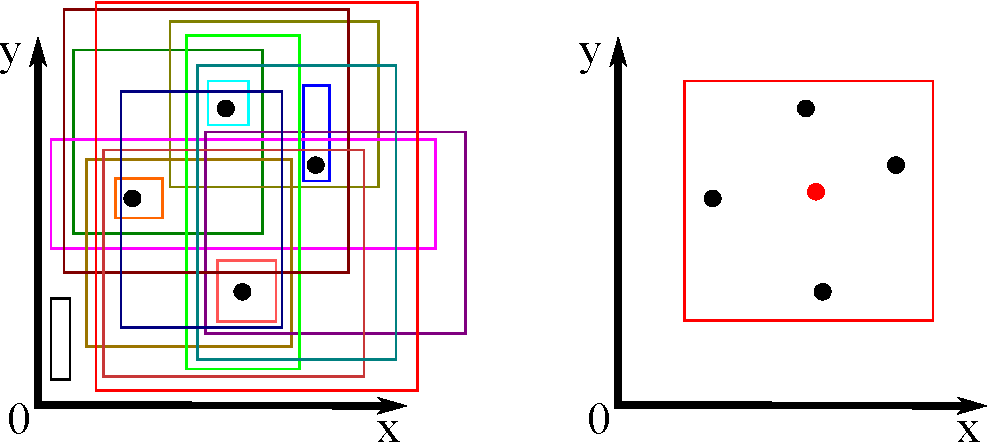
\includegraphics[width=.75\textwidth,keepaspectratio]{prelims/rectangles}
  \caption{Example of range space and VC-dimension. The space of points is the
  plane $\mathbb{R}^2$ and the set $\range$ of ranges is the set of all
  \emph{axis-aligned rectangles}. The figure on the left shows graphically that
  it is possible to shatter a set of four points using 16 rectangles. On the
  right instead, one can see that it is impossible to shatter five points, as,
  for any choice of the five points, there will always be one (the red point in
  the figure) that is internal to the convex hull of the other four, so it would
  be impossible to find an axis-aligned rectangle containing the four points
  but not the internal one. Hence $\VC((\mathbb{R}^2,\range))=4$.}
  \label{fig:rectangles}
\end{figure}

A classic example of a range space with infinite VC-dimension is the space of sine
functions. Let $D=\mathbb{R}^2$ and, for any $\omega\in\mathbb{R}$, let
$A_{\omega}$ be the subset of $\mathbb{R}^2$ that lies \emph{above} the
curve $\sin(\omega t)$, for $t\in \mathbb{R}$. It is possible to
shatter any set $S$ of points by choosing an appropriate $\omega_A$ for each
subset $A\subseteq S$.

Let $\nu$ be a probability distribution on the points of $D$, and let
$X_1^k=(X_1,\dotsc,X_k)$ be a bag of elements from $D$. For any subset
$A\subseteq D$, we define the function 
\[
\nu_{X_1^k}(A)=\frac{1}{k}\sum_{j=1}^k\mathds{1}_A(X_j),\]
where $\mathds{1}_A$ is the indicator function for the set $A$. When $X_1^k$ is
a collection of \emph{independent samples from $\nu$}, then $\nu_{X_1^k}(A)$ is known as the
\emph{empirical average} of $\nu(A)=\sum_{a\in A}\nu(a)$ on $X_1^k$ and is an
\emph{unbiased estimator} for $\nu(A)$ (i.e.,
$\expectation[\nu_{X_1^k}(A)]=\nu(A)$). One of the main applications of
(empirical) VC-dimension is in giving bounds to the number of samples from $\nu$
needed to \emph{simultaneously} approximate the probabilities $\nu(A$) of all
$A\in\range$ using their empirical averages, in the following sense.

\begin{definition}\label{def:eapprox}
  Let $(D,\range)$ be a range space and $\nu$ be a probability distribution on
  $D$. For $\varepsilon\in(0,1)$, an \emph{$\varepsilon$-approximation to
  $(D,\range,\nu)$} is a bag $S$ of elements of $D$ such that 
  \begin{equation}\label{eq:defeapprox}
  \sup_{A\in\range}|\nu(A)-\nu_S(A)|\le\varepsilon\enspace.
\end{equation}
\end{definition}

If $D$ is \emph{finite} and $\nu$ is the \emph{uniform} distribution on $D$, then
$\nu(A)=|A|/|D|$, and~\eqref{eq:defeapprox} is equivalent to
\[
\left|\frac{|A|}{|D|}-\frac{|A\cap S|}{|S|}\right|\le\varepsilon, \forall
A\in\range.
\]
Indeed this will be often but not always the case in later chapters, and we will
simplify the notation by dropping $\nu$ and saying that $S$ is an
$\varepsilon$-approximation to $(D,\range)$.

A great result by~\citet{VapnikC71} showed that it is possible
to compute a $\varepsilon$-approximation with a limited number samples from
$\nu$, provided an upper bound to the VC-dimension of $(D,\range)$ or to its
empirical VC-dimension on a subset of $D$ is known. This result is one of the
reasons why VC-dimension gained fundamental importance in the PAC
framework~\citep{KearnsV94}. The original bound to the number of samples was
improved multiple times. Here we present the most recent improvement.

\begin{theorem}[Thm.~2.12~\citep{HarPS11}, see also~\citep{LiLS01}]\label{thm:eapprox}
  Let $(D,\range)$ be a range space with $\VC(\range)\le d$, and let $\nu$ be a
  distribution on $D$. Given $\varepsilon,\delta\in(0,1)$, let
  %and a positive integer $\ell$, let
  \begin{equation}\label{eq:vceapprox}
  %  \varepsilon = \sqrt{\frac{c}{\ell}\left(d + \log\frac{1}{\delta}\right)}
  \ell = \frac{c}{\varepsilon^2}\left(d + \log\frac{1}{\delta}\right)
  \end{equation}
  where $c$ is an universal constant. Then, a bag of $\ell$ elements of $D$
  sampled independently according to $\nu$ is an $\varepsilon$-approximation to
  $(\range,\nu)$ with probability at least $1-\delta$.
\end{theorem}
The constant $c$ is approximately $0.5$ and it is
\emph{universal}, i.e., it does not depend on any parameter~\citep{LofflerP09}.  
It is also interesting to note that, if $|D|$ is finite, then an
$\varepsilon$-approximation of size
$O(\frac{d}{\varepsilon^2}\log{\frac{d}{\varepsilon}})$ can be built
\emph{deterministically} in time
$O(d^{3d}(\frac{1}{\varepsilon^2}\log{\frac{d}{\varepsilon}})^d|D|)$~\citep{Chazelle00}.

Throughout this dissertation we assume the sample to be drawn \emph{with}
replacement if the sample size is smaller than the size $|D|$ of the domain,
(otherwise the sample is exactly $D$).  

To understand the importance of Thm.~\ref{thm:eapprox}, consider the following
simple example. Assume that $\range$ contains a finite number of ranges and let
$\nu$ be the \emph{uniform} distribution on $D$, and $S$ be a sample of
points drawn uniformly and independently at random (i.e., according to $\nu$)
from $D$. We can compute the sample size $|S|$ needed to obtain an
$\varepsilon$-approximation with probability at least $1-\delta$ by using the
Chernoff bound and the union
bound~\citep{MitzenmacherU05}. Indeed, using the union bound, we have that
\[
\Pr\left(\exists A\in\range ~:~ \left|\nu(A)-\frac{|A\cap
S|}{|S|}\right|>\varepsilon \right) \le \sum_{A\in\range}\Pr\left(\left|\nu(A)-\frac{|A\cap
S|}{|S|}\right|>\varepsilon\right)\]
If the right side is bounded by $\delta$, then $S$ is a
$\varepsilon$-approximation for $(D,\range,\nu)$. A sufficient condition for
this is that, for any $A\in\range$,
\[
\Pr\left(\left|\nu(A)-\frac{|A\cap S|}{|S|}\right|>\varepsilon\right)\le
\frac{\delta}{|\range|}
\]
The quantity
$|A\cap S|$ is a random variable with binomial distribution $B(|S|, \nu(A))$.
Then we can use the Chernoff bound and obtain
\[
\Pr\left(\left|\nu(A)-\frac{|A\cap S|}{|S|}\right|>\varepsilon\right)\le 2e^{-2|S|\varepsilon^2}
\]
which is smaller than $\delta/|\range|$ for
\[
|S|\ge\frac{1}{2\varepsilon^2}\left(\ln|\range|+\ln 2 +\ln\frac{1}{\delta}\right).
\]
Comparing this quantity with~\eqref{eq:vceapprox} clearly shows the multiple
advantages of VC-dimension. Firstly, the sample size suggested
by~\eqref{eq:vceapprox} is smaller than the above as soon as the (upper bound to
the) VC-dimension of $(D,\range)$ is smaller than $\ln(2\range)$ (note that the
above example cannot be used when $\range$ has infinite size). Secondly,
Thm.~\ref{thm:eapprox} holds for \emph{any} distribution $\nu$ and no assumption
are made on it or any of its moments (e.g., on its variance). 
It is important to mention that if $\VC\left((D,\range)\right)$ and/or the upper
bound $d$ do not depend on $|D|$ or on $|\range|$ neither does the sample size
presented in Thm.~\ref{thm:eapprox} (nor the ones in Thm.~\ref{thm:eapproxempir}
and Thm.~\ref{thm:releapprox} which we show next). We use this property in the
following chapters to develop efficient sampling-based randomize algorithms for
important problems in data mining.

It is possible to build an $\varepsilon$-approximation even when only an upper
bound to the empirical VC-Dimension is available.
\begin{theorem}[Sect.~3~\citep{BoucheronBL05}]\label{thm:eapproxempir}
  Let $(D,\range)$ be a range space, and let $\nu$ be a distribution on $D$. Let
  $S$ be a bag of $\ell$ points from $D$ sampled independently according
  to $\nu$. Let $d$ be an integer such that $\EVC(\range,X_1^\ell)\le d$.
  Given $\delta\in(0,1)$, let 
  \begin{equation}\label{eq:evceapprox}
    \varepsilon =
    2\sqrt{\frac{2d\log(\ell+1)}{\ell}}+\sqrt{\frac{2\log\frac{2}{\delta}}{\ell}}.
  \end{equation}
   Then $S$ is a $\varepsilon$-approximation for $(\range,\nu)$
   with probability at least $1-\delta$.
 \end{theorem}

One can define and compute stronger approximations with \emph{relative}
guarantees (rather than additive) as follows.
\begin{definition}\label{def:releapprox}
  Let $(D,\range)$ be a range space  and $\nu$ be a probability distribution on
  $D$. For $p,\varepsilon\in (0,1)$, a \emph{relative
  $(p,\varepsilon)$-approximation to $(D,\range,\nu)$} is a bag $S$ of elements
  from $D$ such that 
  \begin{itemize}
    \item For any $A\in\range$ such that $\nu(A)\ge p$, we have 
      \[ |\nu(A) - \nu_S(A)|\le \varepsilon\nu(A)\enspace.\]
    \item For any $B\in\range$ such that $\nu(B)< p$, we have $\nu_S(B)\le
      (1+\varepsilon)p$.
  \end{itemize}
\end{definition}

\begin{theorem}[Thm.~2.11~\citep{HarPS11}]\label{thm:releapprox}
  Let $(D,\range)$ be a range space with $\VC\left((D,\range)\right)\le d$, and
  let $\nu$ be a distribution on $D$. Given $\varepsilon,\delta,p\in(0,1)$, let 
  \begin{equation}\label{eq:releapprox}
    \ell\ge\frac{c'}{\varepsilon^2p}\left(d\log\frac{1}{p}+\log\frac{1}{\delta}\right)
  \end{equation}
  where $c'$ is an universal constant. Then a bag of $\ell$ points from $D$ sampled
  according to $\nu$ is a relative $(p,\varepsilon)$-approximation to
  $(D,\range,\nu)$ with probability at least $1-\delta$.
\end{theorem}
%No upper bound is currently known for $c'$. 

Up to a constant factor, the bounds presented in Thm.~\ref{thm:eapprox}
and Thm.~\ref{thm:releapprox} are tight~\citep[Thm.~5]{LiLS01}. 

%For any two positive integers  $n>0$ and $d>0$ the {\em growth function}
%$g(d,n)$ is defined as as
%  \[
%  g(d,n)=\sum_{i=0}^d\binom{n}{i} < n^d .\]
%
%If $|D|=n$ and $\VC\left((D,\range)\right)=d$, then $|R|\le g(d,n)$ (Sauer's
%Lemma~\citep[Sect.~14.4]{AlonS08}), hence for every finite $A\subseteq D$,
%$P_\range(A)\le g(d, |A|)$.

%The growth function is used in the following results ~\citep[Sect.~14.4]{AlonS08}.
%\begin{lemma}[Sauer's Lemma]\label{lem:sauer}
%  If $(X,R)$ is a range space of VC-dimension $d$ with $|X|=n$ points, then
%  $|R|\le g(d,n) $.
%\end{lemma}
%\begin{corollary}\label{corol:SauerProj}
%  If $(X,R)$ is a range space of VC-dimension $d$, then for every finite
%  $A\subset X$, $|P_R(A)|\le g(d,|A|)$.
%\end{corollary}

In Sect.~\ref{sec:vcfreqvcdimqueries} we use the following bound
which is an extension of~\citep[Corol.~14.4.3]{AlonS08} to arbitrarily
combinations of set operations. We present it here because it is a general
result on VC-dimension.

\begin{lemma}\label{lem:genboolcomp}
   Let $(D,\range)$ be a range space of VC-dimension $d\ge 2$ and let $(D,\range_h)$ be the
  range space on $D$ in which $\range_h$ includes all possible combinations of 
    union and intersections of $h$ members of $\range$. Then
    $\VC\left((D,\range_h)\right)\le 3dh\log(dh)$.
\end{lemma}

\begin{proof}
  Let $A$ be an arbitrarily subset of cardinality $n$ of $D$.
  From~\citep[Coroll.~14.4.2]{AlonS08}, we have that $|P_\range(A)|\le n^d$. There are 
  \[
  \binom{|P_\range(A)|}{h}\le  n^{dh} \]
  possible choices of $h$ members of $P_\range(A)$, and there are no more
  than $ h! 2^{h-1} C_{h-1}\leq h^{2h}$
  Boolean combinations using unions and intersections of the $h$ sets, where
  $C_{h-1}$ is the $(h-1)^{\mathrm{th}}$ Catalan number
  ($C_i=\frac{1}{i+1}\binom{2i}{i}$). If $2^n> h^{2h}n^{dh} \geq |P_{\range_h}(A)|$
  then $A$ cannot be shattered. This inequality holds for $n\ge 3dh\log(dh)$. To
  see this, consider the fact that clearly $2^n\ge h^{2h}n^{dh}$ for
  sufficiently large $n$, so it suffices to show that $n=3dh\log(dh)$ is
  sufficiently large. Next observe that the function $f(x)=2\log x-\log(3x\log
  x)$ is positive for $x\ge 2$ since it is positive for $x=2$ and it is easy to
  see that the derivative $f'(x)$ is positive for $x\ge 2$. It immediately
  follows that $3\log(dh)> \log(dh)+\log(3dh\log(dh)$ for $d\ge2$ and $h\ge1$.
  Since $dh\log(dh)\ge 2h\log(h)$, we have $3dh\log(dh)> 2h\log(3dh\log(dh))$,
  which proves the result.
\end{proof}

\section{Computational considerations}\label{sec:vccomputcons}
An upper bound to the VC-dimension of the range space is needed in order to
apply Thm.~\ref{thm:eapprox}, Thm.~\ref{thm:eapproxempir}, or
Thm.~\ref{thm:releapprox}. It is natural to ask whether, rather than a bound, one
could compute the exact VC-dimension of a range space. \citet{PapadimitriouY96}
characterized the complexity of computing the VC-dimension. The problem is in
{\sc np}, although it is most probably not {\sc np}-complete. The question is is
whether it can  be solved in polynomial time? \citet{PapadimitriouY96} defined a
new complexity class {\sc lognp} and show that the decision version of the
problem of computing the VC-dimension is {\sc lognp}-complete.
\citet{Schaefer99} showed that in general one can not approximate the problem up
to a constant factor in polynomial time, unless {\sc p}={\sc np}.
\citet{MosselU01} gave a refined characterization of the approximability of the
problem.

\citet{VapnikLLC94}~and~\citet{ShaoCL00} presented and refined an experimental
procedure to estimate the VC-dimension of a learning machine,
and~\citet{McDonaldSS11} gave concentration results for such an estimate. This
procedure is mostly of theoretical interests, as it is computationally very
expensive. It would not be practical in settings like the one we study in this
dissertation, as it would defeat the purpose of using sampling to speed up the
analysis of very large datasets.

